\documentclass[border=10pt]{standalone}
\usepackage{pgfplots}
\pgfplotsset{compat=newest}
\usetikzlibrary{arrows}
\usepgfplotslibrary{fillbetween}

\begin{document}
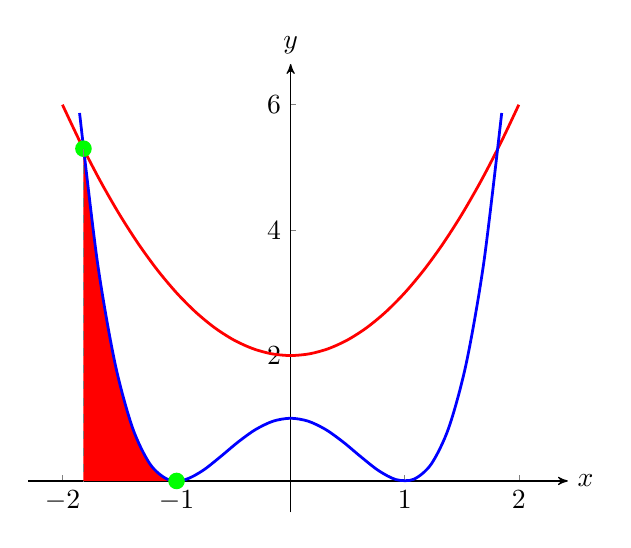
\begin{tikzpicture}[
  declare function={
    f(\x)=pow(\x,2)+2;
    g(\x)=pow(\x,4)-2*pow(\x,2)+1;
  }]
\begin{axis}[
  axis lines*=middle, axis line style={-stealth'}, major tick length=2pt,
  every axis x label/.style={at={(ticklabel* cs:1)}, anchor=west}, 
  xlabel=$x$,
  every axis y label/.style={at={(ticklabel* cs:1)}, anchor=south}, 
  ylabel={$y$},
  enlargelimits=upper, % ticks=none,
  ymin=-0.5, xmin=-2.3,
  ]

  \addplot[red, smooth, domain=-2:2, line width=1, name path=curve_f] {f(\x)};
  \addplot[blue, smooth, domain=-1.85:1.85, line width=1, name path=curve_g] {g(\x)};

  \path[domain=-1.85:0, name path=f(x)_1] plot (\x, {f(\x)});
  \path[domain=-2:0, name path=g(x)_1] plot (\x, {g(\x)});

  \path[name intersections={of=f(x)_1 and g(x)_1, by=A}];
  \node[circle, fill=green, minimum size=6pt, inner sep=0pt] at (A) {};

  \draw[gray, dashed] (A) -- (A |- 0,0);

  \path[name path=base]
    (\pgfkeysvalueof{/pgfplots/xmin},0) --
    (\pgfkeysvalueof{/pgfplots/xmax},0);

  \path[name intersections={of=base and g(x)_1, by=B}];
  \node[circle, fill=green, minimum size=6pt, inner sep=0pt] at (B) {};

  \addplot[red] fill between [of=g(x)_1 and base, soft clip={(A) rectangle (B)}];
\end{axis}
\end{tikzpicture}
\end{document}